	Ever since the Industrial Revolution, the energy consumption of the World has done nothing but rise over time. \cite{owidenergy} This rise in energy consumption correlates well with a rise in quality of life seen throughout the years. \cite{owidQoL} We will therefore take it as an axiom that the continued increase in energy consumption is not only inevitable but also desirable for the Net Good of Humanity. It is worth noting that the distribution of energy consumption and the efficiency of energy consumption are both extremely important topics in and of themselves, but unfortunately are beyond the scope of this discussion. This situation means that energy production must also continue to rise so as to meet the growing demand. \cite{freidberg_plasma_2007}
	
	Unfortunately, time has quickly shown that our current forms of energy production are not sustainable. \cite{owidfossilfuels} The vast majority of energy produced today comes from \emph{fossil fuels}; materials such as coal, oil, and natural gas. \cite{owidenergy} These fuels are formed by natural processes that take place over time periods on the order of millions of years. \cite{sato1990thermochemistry} Due to this extremely long production time, our consumption has far outpaced it leading to these fuels being classified as \emph{non-renewable}. This would not be intrinsically bad if the source was effectively infinite, but most research estimates that these resources can only last on the order of 100 years at current consumption rates. \cite{owidfossilfuels} This finite supply has already lead to a handful of \emph{energy crises} over the years. \cite{bibid}
	
	Even more important than the limited theoretical supply is the environmental impacts of these fuels. Massive amounts of carbon dioxide (CO$_2$) are released into the environment every year due to the burning of fossil fuels. \cite{owidfossilfuels} Research has repeatedly shown that this emission is having harmful, non-reversible impacts on the environment. \cite{ucsusa_fossilfuels, NASA_ClimateChange, stocker_climate_2014} Several countries have deemed this to be undesirable and have taken a variety of actions to reduce future releases of CO$_2$. \cite{paris_treaty} These actions serve to limit the amount of fossil fuels that can be burnt, which even further limits the ability of fossil fuels to meet our growing demand. It is therefore, extremely desirable to develop alternative \emph{renewable} energy sources that can meet our demands without producing exorbitant amounts of CO$_2$.
	
	Thankfully, there are a handful of different energy sources that meet these requirements, each with their own advantages and disadvantages. They are hydroelectric, wind, solar, nuclear fission, and nuclear fusion. 
	
	\subsubsection{Hydroelectric Power}
	
		Hydroelectric power is generated from dams built along the path of rivers. Gravity forces the water to descend through the dam where it passes through and spins a turbine. The spinning turbine drives an electric generator creating the electricity.
		
		\begin{figure}[h!]
			\centering
			\includegraphics[scale=0.175]{Figures/ThreeGorgesDam.pdf}
			\caption[Three Gorges Dam]{The Three Gorges Dam in Sandouping, China is the world's largest power generating station of any kind. It generates 22,500 MW of electricity from the Yangtze River. \cite{cleveland_handbook_2014, ehrlich_renewable_2014, Image_ThreeGorgesDam}}
		\end{figure}
	
		Hydroelectric is considered a renewable resource because the source for a given dam is effectively infinite. Because there is no steam involved, they are highly efficient, only having to convert kinetic energy to electricity. \cite{freidberg_plasma_2007} Dams generate larges amounts of power at competitive costs to fossil fuels \cite{eia_lcoe_2020} and are generally always available. \cite{bibid} Additionally, they can be highly flexible with their power outputs allowing them to follow variable demands. \cite{huggins_energy_2010} All of this without the consequence of releasing CO$_2$ into the environment. \cite{bickel_externe:_2005}
		
		The primary disadvantage of hydroelectric power is the number of suitable locations for dams is finite. While for most countries, there is still room for expansion today \cite{iea_hydro, freidberg_plasma_2007}, it will not be sufficient to meet growing power demands indefinitely. So while hydroelectric is an extremely attractive source of clean renewable energy, it alone cannot serve to meet our energy needs.
		
	
	\subsubsection{Wind Power}
	
		Wind power is generated by large windmills whose blades turn when struck by wind. The spinning blades ultimately turn a turbine which goes on to produce electricity  through an electric motor. 
		
		\begin{figure}[h!]
			\centering
			\includegraphics[scale=0.25]{Figures/windmillFarm.pdf}
			\caption[San Gorgonio Pass Wind Farm]{San Gorgonio Pass Wind Farm located in Riverside County California. The farm consists of 3,218 units delivering a total of 615 MW. \cite{noauthor_awea_2010, Image_WindFarm} }
		\end{figure}
	
		Like hydroelectric, wind is clearly a renewable resource and windmills have no associated CO$_2$ production with operation. \cite{bickel_externe:_2005} Like hydroelectric, no steam is involved in the energy conversion process so it can be made high efficient. \cite{freidberg_plasma_2007}
		
		Wind power does have a handful of disadvantages when compared to fossil fuels. First off, wind is not always available and when it is speeds are variable. This means wind cannot be used as a so called \emph{base load} energy source.\cite{international_energy_agency_variability} Base load sources are those that can produce electricity nearly indefinitely to meet the minimum demand of the grid at all times. \cite{freidberg_plasma_2007} Wind's variable often unpredictable nature means the produced energy often needs to be stored in some way, increasing operational costs. \cite{armaroli_towards_2011} Cost comparisons with fossil fuels vary, but recent estimates show wind power being very competitive with fossil fuels. \cite{eia_lcoe_2020}
		
		All in all, wind is a renewable energy source but has several issues with it's implementation. While it certainly can hold a place in the energy profile of a pure renewable energy grid, it cannot meet the demand reliably alone.
		
	
	\subsubsection{Solar Power}
	
		Solar power largely refers to a variety of technologies that convert radiation from the sun into electricity. \cite{bibid} While the exact method for extracting electricity varies between different technologies, for the purposes of this discussion they largely have the same advantages and disadvantageous.
		
		 \begin{figure}[h!]
		 	\centering
		 	\includegraphics[scale=0.3]{Figures/solarFarm.pdf}
		 	\caption[Serpa solar power plant]{Serpa solar power plant located in Serpa, Portugal. The plant consists of 52,300 units and supplies a total of 11 MW. \cite{noauthor_portugal_2006, Image_SolarFarm}}
		 \end{figure}
	 
	 	Like all the other forms of power generation mentioned thus far, the sun is clearly a renewable source of energy. And like the other renewable sources of energy, no CO$_2$ emissions are required in the conversion to electricity. 
	 	
	 	The disadvantages of solar power are very similar to those discussed with wind power. Solar power only works when the sun is out and even then, can be intermittently interrupted by inopportune weather. \cite{bibid} This makes solar power unattractive as a base load option and necessitates energy storage capabilities. 
	 	
	 	Like wind energy, solar also has a limited energy density. The sun's intensity on earth is about \todo{1.36 kW per square meter} and the efficiency of solar panels is of the order of \todo{15\%}. \cite{bibid} This means you'd need over \todo{1000 square miles} of constant sunlight to power the United States. Accounting for the capability factor brings this estimate up by a factor of 2 or 3. 
	
		Like wind, solar energy certainly has a place but cannot meet the growing energy demand on it's own.
	
	\subsubsection{Nuclear Fission}
	
		Nuclear fission refers to the process of fragmenting large atoms (typically masses of the order 200 amu) into smaller constituents. \cite{bibid} This releases a significant amount of energy (the physics of which we'll discuss in Section \ref{sec:Physics of Nuclear Energy}) which can then be used to heat water and generate electricity through the well known Carnot cycle. \cite{bibid} In fact, the way electricity is produced from nuclear fission is exactly identical to typical fossil fuel plants, the only difference being the source of heat.
		
		\begin{figure}[h!]
			\centering
			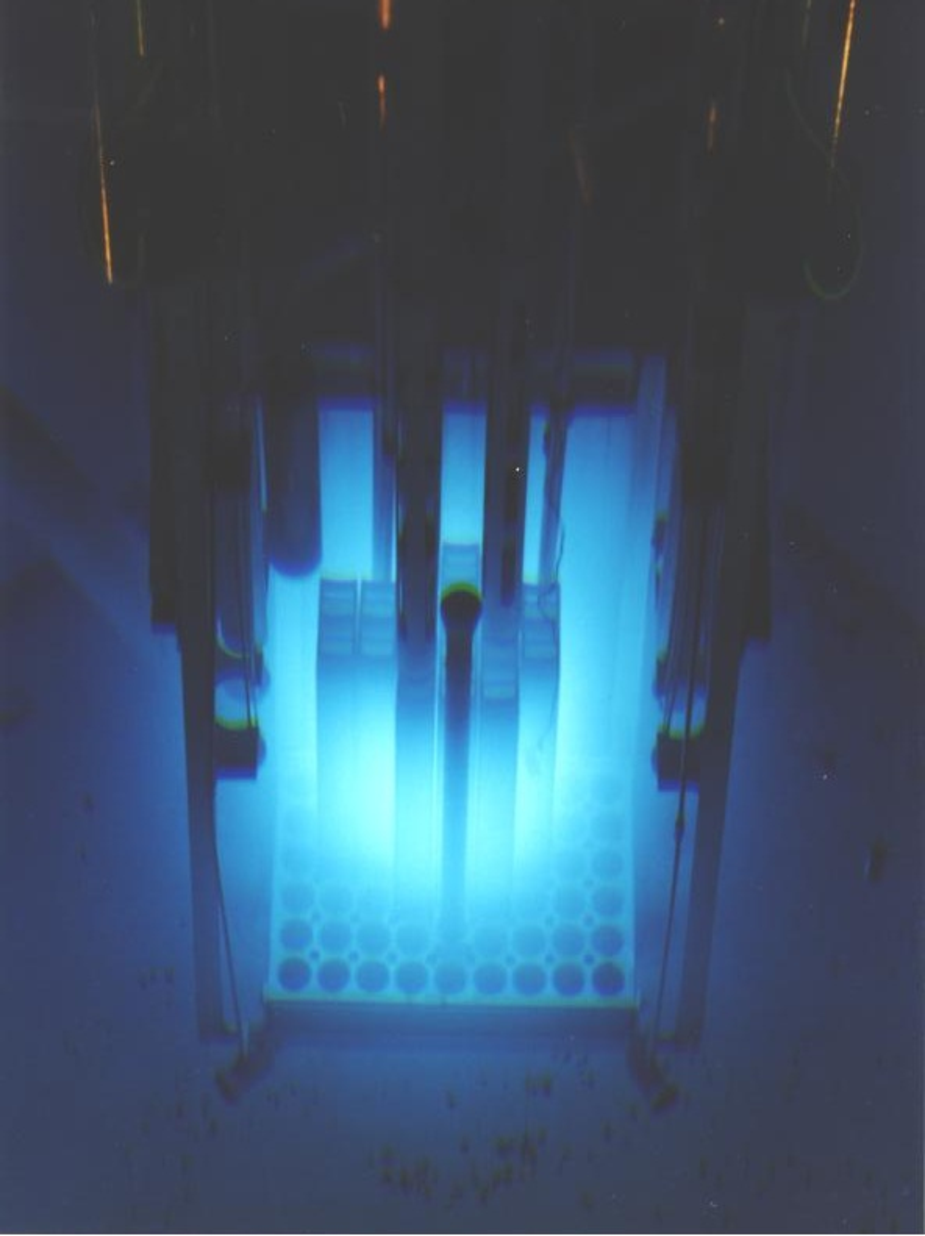
\includegraphics[scale=0.7]{Figures/mstr.pdf}
			\caption[Missouri University of Science \& Technology Nuclear Reactor Core]{Nuclear reactor core of the Missouri University of Science \& Technology Reactor (MSTR). The reactor generates 200 kW of thermal energy and is used primarily for research purposes. The blue glow comes from Cherenkov radiation, caused by high energy electrons being emitted from the fuel with speeds faster than light can travel in water. \cite{tamm1937coherent, Image_MSTR}}
		\end{figure}
		
		When compared to fossil fuels, nuclear fission power has a couple of key advantageous. Firstly, fission generates no CO$_2$ making it a source of clean energy. \cite{bibid} Secondly, the energy density of nuclear fission is orders of magnitude above that of fossil fuels. The potential energy density of UO$_2$ (the fuel used in nuclear reactors) is roughly $7.1\times10^7$ MJ/kg \cite{bibid}. The energy density for coal and methane is only 15 and 55 MJ/kg respectively. \cite{bibid} This means the costs of fuel is practically non-existent for nuclear reactors, with most of the costs being capital cost in constructing the reactor. \cite{bibid} Additionally, the costs of nuclear energy tends to be competitive with fossil fuels when balanced over the life of the reactor. \cite{bibid}
		
		Nuclear fission power also has a couple of advantageous over the traditional renewable energy sources as well. Unlike solar and wind, nuclear power excels as a base load energy production option, often running continuously for 18 months at a time. \cite{bibid} Nuclear power is also traditionally cheaper than solar and wind \cite{bibid}, although over recent years the two have become much more competitive. \cite{bibid} Unlike hydroelectric, expanding nuclear power is only limited by the high investment costs needed to build new plants. 
		
		There are, however, disadvantages associated with nuclear fission power. One is the public perception of it's safety is not remarkable after the accidents at Chernobyl, \cite{bibid} Three Mile Island, \cite{bibid} and Fukushima \cite{bibid}. While there are those that would debate that these examples are unfair representations \cite{bibid}, it is nevertheless true that public opinion continues to be a challenge for nuclear fission. Another disadvantage of this technology is the spent fuel is a extreme radiation hazard have half lives on the order of millions of years. \cite{bibid} While this spent fuel, as of yet, doesn't impact the environment, there is currently no long term plan in the United States on how to handle it. \cite{bibid} 
		
		As noted before, the capital costs of nuclear fission power are much greater than any other energy source. \cite{bibid} Additionally, the act of getting a reactor approved and built is rather lengthy, full of complications, and prone to delays. \cite{bibid} This significantly limits the number of potential investors who can or even who are willing to explore nuclear power. This makes expansion fundamentally difficult. 
		
		Another disadvantage is nuclear fission is (by many accounts) not a true renewable energy source. \cite{bibid} The current most common and cheapest fuel cycles are extremely wasteful. The uranium must be enriched, so only about 10\% of uranium mined out of the ground makes it into the reactor. Of this, roughly 5\% is actually utilized for fission before becoming spent fuel. \cite{https://www.world-nuclear.org/information-library/nuclear-fuel-cycle/introduction/nuclear-fuel-cycle-overview.aspx} Uranium resources used this way at current consumption rates can last on the order of hundreds of years. \cite{bibid} In reality, there are other more efficient fuel cycles that can extend our resources to several thousand years but these come with costs and risks that are beyond the scope of this discussion. \cite{bibid}
		
		One final disadvantage is the concept of nuclear proliferation which, in this context, refers to the idea of a rogue and/or unstable organization acquiring nuclear weapon material somewhere in the fuel cycle. \cite{bibid} In the wasteful cycle we mentioned before, this risk is fairly minimal. However, any efforts to reprocess spent fuel to more efficiently utilize it inherently involves the separation and concentration of plutonium. \cite{bibid} Extreme care must be taken to ensure that none of this plutonium is diverted from the fuel cycle which presents a very real and challenging risk.
		
		In conclusion, nuclear fission power holds extreme promise as an expandable base load power source that does not emit CO$_2$. It does, however, come with a vast amount of non trivial challenges. It certainly will play an important role in any carbon free energy profile, so long as the challenges can be appropriately addressed.
		
		
	\subsubsection{Nuclear Fusion}
	
		Nuclear fusion is very similar to nuclear fission except it involves combining light atoms (masses of order 1 amu) together. \cite{bibid} Like with fission, this generates enormous amounts of energy which could be used as a heat source in any variety of thermodynamic cycles. Unlike with the other technologies discussed thus far, nuclear fusion power has yet to be scientifically demonstrated. \cite{bibid}
		
		\begin{figure}[h!]
			\centering
			\includegraphics[scale=0.1]{Figures/sol.pdf}
			\caption[The Sun]{False-color image of the Sun taken at 304 angstroms. It is the star at the center of the Solar System. The Sun's power comes from the nuclear fusion of hydrogen atoms forced to extreme temperatures and pressures due to the Sun's own gravity. \cite{woolfson_origin_2000, Image_Sun}}
		\end{figure}
		
		Nuclear fusion shares many of the advantages of nuclear fission. Like fission, nuclear fusion power would emit no CO$_2$ into the environment and it has an extremely high fuel energy density. If one were to consider the fusion of hydrogen isotopes tritium (T) and deuterium (D), the energy density is of order 3.5 MeV per amu compared to fission of $^{235}$U which is more like 0.85 MeV per amu. \cite{bibid} It's also possible to simply fuse D with D which is found in trace amounts in water (H$_2$O). With this in mind, a perhaps more fair comparison is the potential fusion energy density of H$_2$O which is roughly $3\times10^3$ MJ/kg; still orders of magnitude above coal and methane. \cite{bibid}
		
		Like hinted at, the primary source of fuel for any nuclear fusion power scheme would be hydrogen. There are other reactions that would involve other fuels such as helium or even boron, but we shall ignore those for now. \cite{bibid} Deuterium is naturally present in water of which there is a significant abundance on Earth. \cite{bibid} Any fusion power plant that used deuterium alone would certainly be considered effectively renewable due to the massive water reserves available in oceans. In reality, the first generation of nuclear fusion reactors would rely on tritium which does not exist naturally on Earth. It can, however, be produced from $^6$Li or even deuterium via neutron bombardment. \cite{bibid} Thankfully, lithium is also plentiful on Earth, not so much as to be considered renewable, but enough that it could last tens of thousands of years at current electrical consumption rates. \cite{bibid} 
		
		A unique advantage of nuclear fusion is it's intrinsic safety. The reason fusion power has yet to be scientifically demonstrated is exactly the same thing that makes it so safe. Nuclear fusion requires the containment of fuel hotter than the center of the Sun, which is an extreme scientific and engineering challenge. \cite{bibid} While this may sound unsafe, it means that the these extreme temperatures must be maintained for the fusion reaction to continue. Any failure mode that would result in a compromised containment which would immediate halt any additional fusion reactions. In addition, by design, fusion reactors only have very small amounts of fuel in the "core" at any given time. This is distinctly different from fission where a reactor is loaded with enough fuel such that 5\% of it will last 18 months. \cite{bibid}.  What this means is that even if all of the fusion fuel were to be consumed in a runaway reaction, the total energy released would be minimal. In Inertial Confinement Fusion (ICF) schemes, all of the fuel in current designs translates to roughly 100 sticks of dynamite which is certainly containable with modern containment structures. \cite{bibid}
		
		Another advantage that nuclear fusion would have over nuclear fission, is the lack of long lived radioactive spent fuel. For fusion, the spent fuel is generally some combination of hydrogen and helium both of which are completely inert to the environment. \cite{bibid} In the case of DD fusion, the spent fuel would actually be radioactive (in the form of tritium), but the half-life is on the order of 10 years, not millions. \cite{bibid} Nuclear fusion does emit high energy neutrons that would go on to activate structural materials. These activated structural materials would half half-lives on the order of hundreds of years, again much lower than that of spent fuel from nuclear fission. \cite{bibid}
		
		The primary disadvantage of nuclear fusion is quite clear; the technology does not exist. Unlike with nuclear fission power, nuclear fusion power has been out of reach for nearly 70 years. \cite{bibid} This is because the technical demands associated with trying to contain a plasma hotter than the Sun here on Earth is quite challenging. To date, the technical viability of fusion has never been demonstrated outside of nuclear weapons and, infact, many attempts have failed. \cite{bibid} All of that said, the performance of nuclear fusion experiments has shown a steady increase over time suggesting that success will come inevitably. \cite{bibid}
		
		Another very real disadvantage of nuclear fusion is the expected costs. Nuclear fusion facilities are currently very expensive to operate and would never be able to generate electricity competitively. \cite{bibid} For example, the National Ignition Facility (NIF) spends roughly \todo{one million USD} per experiment. \cite{bibid} The maximum theoretical yield from one of these experiments would generate less than 6 USD worth of electricity at current costs. \cite{bibid} Using instead the maximum credible yield combined with the fact that energy will be loss converting to electricity brings this estimate below 1 USD. \cite{bibid} While technology will expected to lower costs over time and electricity prices are likely to rise, the fact remains that the current gap is many orders of magnitude away.
		
		In summary nuclear fusion power holds great potential as a future base load power source with seemingly no safety risk or negative consequences. It's potential is locked entirely by technical and scientific issues that require more study and research. While nuclear fission is certainly sufficient to supply to World's clean energy needs in years to come, the vast potential of nuclear fusion justifies it's continued investigation. We will therefore spend the introduction of this thesis discussing the basic theory and the current state of nuclear fusion efforts. 